\chapter{Teaching Experiments and Computational Experiments}
\label{chap:e26}

\begin{chapteropening}
Up to this point we have built the whole language: photon arrivals are a random point process (Chapter \ref{chap:e03}), thermal light \textbf{bunches} while coherent light does not (Chapter \ref{chap:e08}), the degree of spatial coherence between two telescopes is the visibility of the object's brightness distribution (Chapters \ref{chap:e10}, \ref{chap:e11}), and the information about some parameters is simply not in the plot you are most used to looking at (Chapter \ref{chap:e12}). Being told these truths once is one thing; \textbf{computing them yourself, seeing them, and knowing where they will fool you} is another. This chapter is that laboratory. We do not hand out a pile of ready-to-run code; instead we break each key concept into a \textbf{recomputable experiment chain}: starting from a simulated photon event table, seeing how it becomes a statistic, how the statistic enters a physical model, and how the model's error in turn forces you to redesign the experiment. Along the way you will use simulated data to verify Poisson statistics and bunching with your own eyes, numerically demonstrate how SPADE crosses the Rayleigh limit, fit the visibilities of a uniform disk and a binary, and finally assemble these parts into a toy model for Type Ia supernova ranging. Each experiment comes with one line of ``common pitfall,'' because in this line of work, a curve that is too pretty is often not good news but an undiscovered error.
\end{chapteropening}

\section{The event table: the shared draft of all computational experiments}
\label{sec:e26-eventtable}

First set the scene. The starting point of all experiments in this chapter is an \textbf{event table}: not some deep data structure, just a table, each row recording one photon: when it arrived (time stamp \(t_i\)), which detector or channel it fell in, what its polarization was, and a ``quality flag'' \(q_i\) saying whether this photon can be trusted (whether it falls near dead time, whether it was blocked by a cloud, whether the electronics saturated). Chapter \ref{chap:e13} explained why we must store it this way: once you first coarsely bin photons in time and connect them into a smooth \textbf{light curve}, you can no longer go back to re-select time windows, re-filter by polarization or energy channel, or re-do a time-shifted background estimate. Binning is a form of \textbf{lossy compression}. The event table, by contrast, keeps the randomness of the light field intact on disk.

Real photon-counting instruments work exactly this way. Devices like AQuEye and IquEye keep every photon as a time tag, with time resolution down to tens of picoseconds and absolute time constrained by GPS or an atomic clock to the nanosecond or even sub-nanosecond level; pixel-counting chips like Timepix even let each row simultaneously carry spatial position and energy information \citep{2016SPIE.9907E..0NZ,2015SPIE.9504E..0CZ,2007NIMPA.581..485L}. So the first discipline of this chapter is: \textbf{experiments begin from the event table, not from the light curve}.

If you truly care only about the light curve, that too is simple: just project the event table onto time bins:
\begin{equation}
  n_k=\sum_i \mathbf 1\!\big(t_i\in[t_k,\,t_k+\Delta t)\big)\,\mathbf 1\!\big(q_i=1\big).
  \label{eq:e26-binned-count}
\end{equation}
\begin{formulaexplain}
\(n_k\) is the number of photons in the \(k\)-th time bin that ``pass quality selection.'' The two indicator functions \(\mathbf 1(\cdot)\) act like two gates: the first checks whether the photon's arrival time falls in this bin, and the second checks whether the photon's quality is acceptable (only \(q_i=1\) passes). The sum counts how many photons pass both gates at once.
\end{formulaexplain}
Grounding the units and dimensions symbol by symbol: \(n_k\) is a pure count, dimensionless; \(\Delta t\) is the bin width (units s), often taken from nanoseconds to milliseconds in tabletop experiments, and from nanoseconds to minutes in astronomical timing; \(\mathbf 1(A)\) is the indicator function, taking 1 if condition \(A\) holds and 0 otherwise. To turn it into a photon rate, simply take \(r_k=n_k/\Delta t\), with units \(\mathrm{s^{-1}}\). A pitfall is already buried here: when each bin has on average only a few to a few tens of photons, the count fluctuation is Poisson, and one \textbf{cannot} casually replace it with symmetric Gaussian error bars; only once \(n_k\gtrsim30\) is the Gaussian approximation roughly usable. Equation \eqref{eq:e26-binned-count} looks bland, but it is the first step of every experiment in this chapter: first have the event table, then decide what to project it into.

\begin{figure}[tbp]
\centering
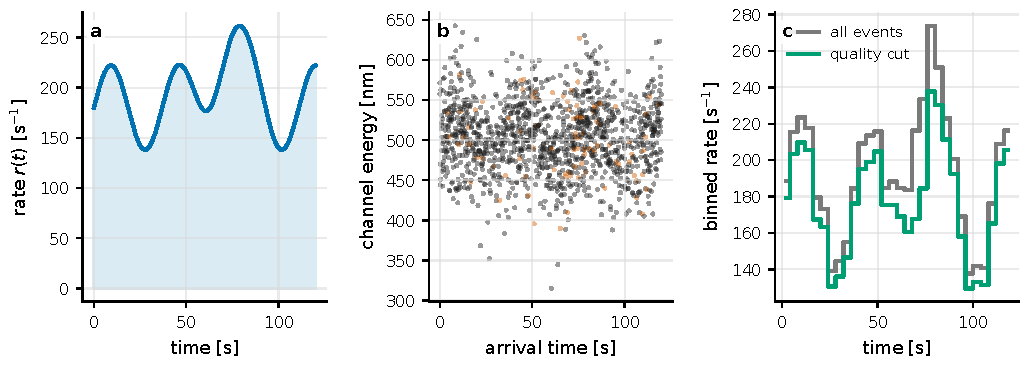
\includegraphics[width=0.96\linewidth]{figures/generated/chapter_20/ch20_event_table_simulation.pdf}
\caption{A simulated event table generated by an inhomogeneous Poisson process. The left panel is the input photon rate \(r(t)\); the middle panel retains each photon's arrival time, equivalent wavelength channel, and quality flag; the right panel projects the event table into a light curve and shows the effect of quality selection. The event table keeps channel and quality information beyond the light curve, so the same data can still be re-used for correlation, polarization, or energy-spectrum analysis.}
\label{fig:e26-eventtable}
\end{figure}

\section{The first computational experiment: build an event table, verify Poisson and shot noise}
\label{sec:e26-poisson}

The goal of the first experiment is the plainest yet the most important: \textbf{build by hand an event table that obeys Poisson statistics, then use it to verify Poisson statistics back}, thereby thoroughly digesting the shot noise of Chapter \ref{chap:e03}.

First, ``how to build.'' If the photon rate is constant at \(r\), the most economical way is to use a property of the Poisson process: the time interval between two adjacent photons follows an exponential distribution, \(P(\Delta t)=r\,e^{-r\Delta t}\). So from a uniform random number \(u\in(0,1)\) take \(\Delta t=-\ln(u)/r\), accumulate one after another, and obtain a string of arrival times. If the rate varies with time, \(r(t)\) (as in the left panel of Figure \ref{fig:e26-eventtable}), use \textbf{thinning}: first generate candidate photons at a constant rate \(r_{\max}\) higher than all times, then for each candidate independently ``keep or discard'' with probability \(r(t_i)/r_{\max}\). Those kept are one true realization of the inhomogeneous Poisson process. The virtue of this method is that it forces you to think through ``where the randomness comes from'' rather than tuning a black-box function.

Now verify. At constant rate, the number of photons \(N\) in a bin of length \(\Delta t\) follows the Poisson distribution, a known result of Chapter \ref{chap:e03}, used here by name:
\begin{equation}
  P(N)=\frac{\mu^{N}}{N!}\,e^{-\mu},\qquad \mu=r\,\Delta t .
  \label{eq:e26-poisson-pmf}
\end{equation}
\begin{formulaexplain}
\(P(N)\) is the probability of counting exactly \(N\) photons in a bin, and \(\mu\) is the \textbf{mean} photon number of this bin (equal to rate times bin width). The Poisson distribution is determined by the single parameter \(\mu\), which is both its mean and its variance, its most useful and most testable property.
\end{formulaexplain}
Grounding the symbols: \(N\) is a dimensionless count, \(\mu=\bar N\) is the dimensionless mean count, \(r\) has units \(\mathrm{s^{-1}}\), and \(\Delta t\) has units s. The place where the Poisson distribution can be verified at a glance is that its mean and variance are \textbf{equal}. We write this as a test quantity computable directly from data: the \textbf{Fano factor}:
\begin{equation}
  F=\frac{\operatorname{Var}(N)}{\langle N\rangle}\;\xrightarrow[\text{Poisson}]{}\;1 .
  \label{eq:e26-fano}
\end{equation}
\begin{formulaexplain}
\(\langle N\rangle\) is the sample mean of the bin counts, and \(\operatorname{Var}(N)\) is their sample variance. The Fano factor \(F\) is the ratio of the two. Pure Poisson (coherent light, shot-noise-dominated) gives \(F=1\); bunched thermal light gives \(F>1\), and antibunched nonclassical light gives \(F<1\).
\end{formulaexplain}
Why is the Poisson variance exactly equal to the mean? This is no coincidence and is worth deriving on the spot. From Eq.\ \eqref{eq:e26-poisson-pmf},
\[
  \langle N\rangle=\sum_{N=0}^{\infty}N\,\frac{\mu^N}{N!}e^{-\mu}
  =\mu\,e^{-\mu}\sum_{N=1}^{\infty}\frac{\mu^{N-1}}{(N-1)!}
  =\mu\,e^{-\mu}\,e^{\mu}=\mu,
\]
where we used the \textbf{exponential series expansion} \(\sum_{m\ge0}\mu^m/m!=e^{\mu}\) (substituting \(m=N-1\)). Similarly compute the second factorial moment:
\[
  \langle N(N-1)\rangle=\sum_{N=0}^{\infty}N(N-1)\frac{\mu^N}{N!}e^{-\mu}
  =\mu^2 e^{-\mu}\sum_{N=2}^{\infty}\frac{\mu^{N-2}}{(N-2)!}=\mu^2 .
\]
So \(\langle N^2\rangle=\langle N(N-1)\rangle+\langle N\rangle=\mu^2+\mu\), and substituting into the variance definition:
\[
  \operatorname{Var}(N)=\langle N^2\rangle-\langle N\rangle^2=(\mu^2+\mu)-\mu^2=\mu .
\]
The variance equals the mean, with not a step skipped. This is the origin of the famous shot-noise line ``\(\sigma_N=\sqrt{\bar N}\),'' and the basis of \(F\to1\) in Eq.\ \eqref{eq:e26-fano}.

Order of magnitude: if the event table you build has mean rate \(r=5\times10^{5}\,\mathrm{s^{-1}}\) and bin width \(\Delta t=1\,\mathrm{ms}\), then each bin has \(\mu=500\) photons, with relative fluctuation \(1/\sqrt{\mu}\simeq4.5\%\); shrink the bin width to \(1\,\mu\mathrm{s}\) and \(\mu=0.5\), most bins are empty, and the Fano test relies on the statistics of a large number of bins to be stable. \textbf{Common pitfall}: if you compute an \(F\) clearly deviating from 1, do not rush to declare that you have seen nonclassical light: more likely the detector \textbf{dead time} is at work. Dead time briefly ``blinds'' the detector after a photon, suppressing closely following counts and thereby artificially pushing the variance below the mean (\(F<1\)), disguising itself as antibunching. So this most basic experiment is in fact teaching you to distinguish ``physics'' from ``instrument.''

\section{Tabletop HBT: ``seeing'' bunching amid random coincidences}
\label{sec:e26-hbt}

The second experiment pushes Poisson to \textbf{second order}: with one beam of light, one beamsplitter, and two detectors, do a tabletop version of the Hanbury Brown--Twiss (HBT) experiment, measure \(g^{(2)}(\tau)\) by hand, and verify the bunching of Chapter \ref{chap:e08} \citep{1956Natur.178.1046H,1957RSPSA.242..300B,1963PhRv..130.2529G}.

First the picture. Each of the two intensity streams jitters randomly; why should there be a bit more ``common'' fluctuation near zero delay than elsewhere? Think of thermal light (or the \textbf{pseudothermal light} made by a rotating ground glass) as a superposition of many random-phase modes; its instantaneous intensity is not flat but jumps up and down. Within one \textbf{coherence time} \(\tau_c\), this one intensity fluctuation is \textbf{shared} by both detectors: in the instant of high intensity, both sides are more likely to each receive a photon, so ``coincidences'' increase near \(\tau=0\). Laser light is the exception: each of its modes is phase-locked, and the intensity is flat as a stagnant pool, so \(g^{(2)}(0)\simeq1\), no bunching \citep{1991PhRvL..67.1426N,1999PhRvA..60..674B,2024arXiv240418606N}.

How do we compute it from the event table? The method is to count \textbf{coincidence pairs} and normalize. Bin the two event tables by time difference \(\tau=t_j^{(2)}-t_i^{(1)}\) into a delay histogram \(H(\tau)\), then divide by an ``as-expected'' random baseline:
\begin{equation}
  \hat g^{(2)}(\tau)=\frac{H(\tau)}{H_{\rm bg}(\tau)},\qquad
  H_{\rm bg}\simeq R_1 R_2\,T\,\Delta\tau .
  \label{eq:e26-g2-estimator}
\end{equation}
\begin{formulaexplain}
\(H(\tau)\) is the number of photon pairs whose time difference falls in the \(\tau\)-th delay bin. \(H_{\rm bg}\) is the number of accidental coincidences there ``should'' be if the two streams were completely independent: the two rates \(R_1,R_2\) multiplied, times the total duration \(T\), times the delay-bin width \(\Delta\tau\). Dividing cancels the instrument's absolute counts, leaving only the excess \textbf{relative} to random coincidences.
\end{formulaexplain}
Grounding the symbols: \(R_1,R_2\) are the two single-count rates (\(\mathrm{s^{-1}}\)), \(T\) is the total integration time (s), \(\Delta\tau\) is the delay-bin width (s), and \(H,H_{\rm bg}\) are both dimensionless counts. The denominator \(H_{\rm bg}\) has a more reliable measured version: shift the second stream as a whole by an amount far greater than \(\tau_c\) and count coincidences again: by then the physical correlation has long vanished and what remains is purely accidental, which is the \textbf{time-shift background}. Normalizing by it automatically absorbs slow drifts.

The order of magnitude should give one confidence. Take \(R_1=R_2=5\times10^{5}\,\mathrm{s^{-1}}\), \(T=300\,\mathrm{s}\), \(\Delta\tau=0.5\,\mathrm{ns}\); then the accidental coincidences per delay bin are about
\[
  H_{\rm bg}\simeq (5\times10^5)^2\times300\times(0.5\times10^{-9})\approx3.75\times10^{4}\ \text{pairs/bin}.
\]
These pair counts themselves fluctuate as Poisson, with relative shot error about \(1/\sqrt{H_{\rm bg}}\simeq5\times10^{-3}\). So a peak of \(g^{(2)}-1\sim10^{-2}\) is visible above the noise on the tabletop, and this is exactly where the problem lies.

\begin{figure}[tbp]
\centering
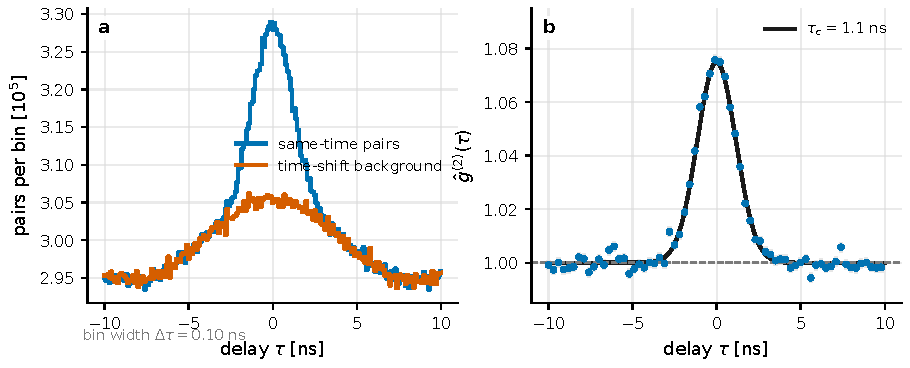
\includegraphics[width=0.96\linewidth]{figures/generated/chapter_20/ch20_hbt_lab_histogram.pdf}
\caption{The delay histogram of tabletop HBT. The left panel compares ``pairs/bin'' on the simultaneous time axis with the time-shift background; slow drifts appear in both curves and are therefore canceled by normalization. The right panel gives \(\hat g^{(2)}(\tau)\) after normalizing by the background histogram, with the peak width near zero delay set jointly by the source coherence time and the detector response.}
\label{fig:e26-hbt}
\end{figure}

\textbf{The deadliest pitfall: contrast dilution.} What a real instrument measures is not the ideal \(g^{(2)}\) but its shape after being \textbf{convolved} by the detector time response. If the coherence time \(\tau_c\) is far smaller than the electronics response width or the delay-bin width \(\Delta\tau\), the peak that thermal light should reach at 2 gets diluted, and the observed contrast shrinks approximately as \(\tau_c/\Delta\tau\). Here is the computation: a narrowband filter centered at \(416\,\mathrm{nm}\) with bandwidth \(\Delta\lambda=13\,\mathrm{nm}\) converts to \(\Delta\nu\simeq c\,\Delta\lambda/\lambda^2\approx2.3\times10^{13}\,\mathrm{Hz}\), so \(\tau_c\simeq1/\Delta\nu\approx4\times10^{-14}\,\mathrm{s}\); sampling with electronics of a few nanoseconds, the contrast is suppressed to \(\tau_c/\Delta\tau\sim10^{-5}\) in magnitude. This is why, if you see a tall, pretty peak on the tabletop, your first reaction should \textbf{not} be delight but the question: does it come from single-mode thermal light, or from electronics crosstalk, source slow drift, or a normalization chosen too conveniently? The intensity-interferometry analyses of VERITAS, MAGIC, and Asiago all, without exception, must explicitly handle this ledger of dilution, background, and dead time \citep{2009A&A...508..531N,2020NatAs...4.1164A,2024MNRAS.529.4387A,2017MNRAS.472.4126G}. This also incidentally explains the division of labor of the next section: the \(10^{-2}\) peak visible on the tabletop and the \(10^{-5}\) peak that must be dug out astronomically differ by five orders of magnitude.

\section{From tabletop to long baseline: simulating and fitting the uniform-disk visibility}
\label{sec:e26-disk}

Move HBT from the tabletop to between \textbf{two telescopes}, and it becomes an intensity interferometer (Chapter \ref{chap:e10}). The physics has not changed, still comparing whether two intensity streams fluctuate in sync, but now the two telescopes look at the same star of \textbf{finite angular size}. The longer the baseline, the more differently the two apertures see the coherent fluctuations, and the lower the zero-delay peak. This ``falling with baseline'' curve is precisely the visibility of the object's brightness distribution.

The Siegert relation of Chapter \ref{chap:e08} tells us that the excess of the second-order correlation equals the modulus squared of the first-order degree of coherence; the van Cittert--Zernike theorem of Chapter \ref{chap:e10} in turn tells us that the first-order spatial coherence \(\gamma_{12}\) between two telescopes is the Fourier transform of the object's normalized brightness distribution, that is, the visibility \(V\). Joining the two, the experimental procedure for estimating \(|V|^2\) from data is this: each baseline \(b\) first gives the zero-delay excess correlation \(\hat c_b=\hat g^{(2)}_b(0)-1\), then divides by the instrument contrast \(\hat\beta_b\) measured from that night's calibration star (or laboratory calibration):
\begin{equation}
  \widehat{|V_b|^2}=\frac{\hat c_b}{\hat\beta_b}.
  \label{eq:e26-v2-estimator}
\end{equation}
\begin{formulaexplain}
\(\hat c_b\) is the zero-delay excess correlation measured on baseline \(b\), and \(\hat\beta_b\) is the instrument contrast of the same baseline (folding in the dilution from time response, bandwidth, polarization selection, and efficiency). Dividing the two extracts the object's own \(|V_b|^2\). Note: \(\beta\) appears in the \textbf{denominator}, so its calibration error is \textbf{directly amplified} into the result.
\end{formulaexplain}
\(\hat c_b\), \(\hat\beta_b\), and \(|V_b|^2\) are all dimensionless. If a baseline's accidental-coincidence count is \(H_b\) and systematic error is momentarily ignored, then \(\sigma_{\hat c}\simeq H_b^{-1/2}\); but once the true contrast is as small as \(\beta\sim10^{-5}\), the same \(\sigma_{\hat c}\) is amplified into \(\sigma_{|V|^2}\simeq\sigma_{\hat c}/\beta\). \textbf{The pitfall of teaching simulations is precisely here}: to make the signal visible on the plot, you will be tempted to set \(\beta\) to a ``friendly'' value like \(0.05\), obtaining a \(g^{(2)}\) peak that pretends to be very clean; but the precision of the real astronomical \(|V|^2\) is still set by that true contrast of \(10^{-6}\)--\(10^{-5}\), the accidental-coincidence count, and the systematic floor. Writing this amplification factor in the most conspicuous place of the report when doing simulations is basic honesty.

Now build data and fit. The most commonly used source model is the \textbf{uniform disk}, whose visibility is the known result of Chapter \ref{chap:e11}, used by name:
\begin{equation}
  V(B_\perp)=\frac{2J_1(x)}{x},\qquad
  x=\frac{\pi\,\theta\,B_\perp}{\lambda},
  \label{eq:e26-uniform-disk}
\end{equation}
\begin{formulaexplain}
\(V\) is the visibility, \(J_1\) is the first-order Bessel function, and \(x\) is a dimensionless combination of angular diameter, baseline, and wavelength. The larger \(x\) (longer baseline or larger star), the smaller \(V\); \(2J_1(x)/x\) tends to 1 as \(x\to0\), and first vanishes at \(x=3.8317\). What one can obtain observationally is \(|V|^2\); the sign of the phase information is lost in intensity interferometry.
\end{formulaexplain}
Grounding each symbol: \(\theta\) is the angular diameter (rad, often written mas or \(\mu\mathrm{as}\) in reports), \(B_\perp\) is the projected baseline (m), \(\lambda\) is the observing wavelength (m), and \(J_1\) is dimensionless. Substituting the first zero \(x=3.8317\) gives the baseline most sensitive to angular diameter:
\[
  B_{\rm null}=\frac{3.8317}{\pi}\,\frac{\lambda}{\theta}\approx1.22\,\frac{\lambda}{\theta}.
\]
Plugging in real numbers: \(\lambda=416\,\mathrm{nm}\), \(\theta=1\,\mathrm{mas}=4.85\times10^{-9}\,\mathrm{rad}\),
\[
  B_{\rm null}\approx1.22\times\frac{416\times10^{-9}}{4.85\times10^{-9}}\ \mathrm{m}\approx105\,\mathrm{m}.
\]
This one number explains the whole landscape: the first zero of a \(1\,\mathrm{mas}\) bright star falls on a hundred-meter baseline, which is why hundred-meter-scale Cherenkov arrays like VERITAS can measure bright-star angular diameters; whereas the few-\(\mu\mathrm{as}\) angular radius of a Type Ia supernova pushes the first zero out to tens of kilometers, reachable only by kilometer-scale baselines. The \textbf{key point} when fitting is: \(|V|^2\) is most sensitive to \(\theta\) on the steep slope near the first zero, so if the baseline coverage all crowds into the \(V\approx1\) plateau region, the posterior will be very wide; spread the baselines to both sides of the zero and the angular diameter tightens up.

\begin{figure}[tbp]
\centering
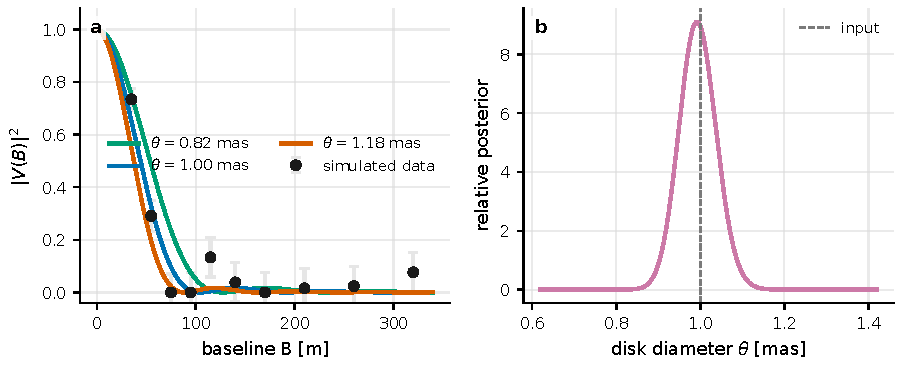
\includegraphics[width=0.96\linewidth]{figures/generated/chapter_20/ch20_uniform_disk_fit.pdf}
\caption{Intensity-interferometry fit of a uniform disk. The left panel simulates \(|V|^2\) measurements at various baselines for a target with \(\lambda=416\,\mathrm{nm}\), \(\theta=1\,\mathrm{mas}\); the slope is greatest and most sensitive to angular diameter near the first zero. The right panel converts these data into the angular-diameter posterior, whose width is set jointly by the \(|V|^2\) error, the baseline coverage, and the model assumptions.}
\label{fig:e26-disk}
\end{figure}

\section{Binaries and uv coverage: why multiple baselines and multiple epochs}
\label{sec:e26-binary}

The uniform disk has only one parameter; a binary makes the story interesting: it lets you see with your own eyes that although intensity interferometry loses the visibility's \textbf{sign} (phase), it still retains the \textbf{spatial frequency} that oscillates with baseline. The normalized squared visibility of two incoherent point sources is the known result of Chapters \ref{chap:e10}, \ref{chap:e11}:
\begin{equation}
  |V(\bm B_\perp)|^2=\frac{1+\rho^2+2\rho\cos\!\big(2\pi\,\bm B_\perp\!\cdot\!\bm s/\lambda\big)}{(1+\rho)^2},
  \label{eq:e26-binary}
\end{equation}
\begin{formulaexplain}
\(\rho=F_2/F_1\) is the flux ratio of the companion to the primary, \(\bm s\) is the angular-separation vector of the two stars, and \(\bm B_\perp\!\cdot\!\bm s/\lambda\) is the dimensionless phase projected onto the baseline direction. The cosine term in the numerator makes \(|V|^2\) oscillate along the baseline, and the denominator \((1+\rho)^2\) merely normalizes it to 1 at \(\bm B_\perp\to0\).
\end{formulaexplain}
Grounding the symbols and dimensions: \(\rho\) is dimensionless, \(\bm s\) is an angular vector (rad, often mas in reports), \(\bm B_\perp\) has units m, \(\lambda\) has units m, and the whole \(\bm B_\perp\!\cdot\!\bm s/\lambda\) is dimensionless. Look at two extremes to feel what it says. For an equal-brightness binary \(\rho=1\), Eq.\ \eqref{eq:e26-binary} reduces to \((1+\cos\phi)/2\), swinging from 1 all the way to 0 with phase: full modulation. If the companion has only a tenth of the primary's flux, \(\rho=0.1\), the cosine term makes \(|V|^2\) swing up and down about its mean, and this \textbf{oscillation half-amplitude} is
\[
  \frac{2\rho}{(1+\rho)^2}=\frac{2\times0.1}{1.1^2}\approx0.17,
\]
while the center of the swing (the mean) is \(\dfrac{1+\rho^2}{(1+\rho)^2}=\dfrac{1.01}{1.21}\approx0.835\). So \(|V|^2\) swings \(0.17\) on either side of the mean \(0.835\), actually rippling between about \(0.67\) and \(1\): the maximum \(1\) occurs at \(\cos\phi=1\), and the minimum \(\dfrac{(1-\rho)^2}{(1+\rho)^2}=\dfrac{0.81}{1.21}\approx0.67\) at \(\cos\phi=-1\), a peak-to-trough difference of about \(0.33\). The fainter the companion, the shallower the ripple, and the more it tests measurement precision. Compute the phase too: with \(B=180\,\mathrm{m}\), \(\lambda=500\,\mathrm{nm}\), separation \(0.5\,\mathrm{mas}=2.42\times10^{-9}\,\mathrm{rad}\),
\[
  \phi=2\pi\frac{B\,s}{\lambda}=2\pi\times\frac{180\times2.42\times10^{-9}}{500\times10^{-9}}\approx5.5\ \mathrm{rad},
\]
close to a full turn: a clear single oscillation period is visible on a single baseline.

But one baseline is only \textbf{one point} in the uv plane (Chapter \ref{chap:e11}). To simultaneously determine the magnitude and direction of the separation, the flux ratio, and the orbital geometry, one must spread out the uv coverage: multiple baselines sample different \(\bm B_\perp\) at a given instant, Earth rotation makes each baseline's projection \(\bm B_\perp(t)\) trace an arc over a night (\textbf{Earth-rotation aperture synthesis}), and multiple epochs let \(\bm s(t)\) sweep through different phases with orbital motion. This is the substance of the slogan ``multiple baselines, multiple epochs'': \textbf{use different uv samplings to pull apart the degenerate parameters one by one}. \textbf{Common pitfall}: if the uv coverage lies along only one direction, the separation in the perpendicular direction is essentially unconstrained, and the fit gives an elongated, misleading error ellipse: a nice-looking plot with untrustworthy parameters.

\begin{figure}[tbp]
\centering
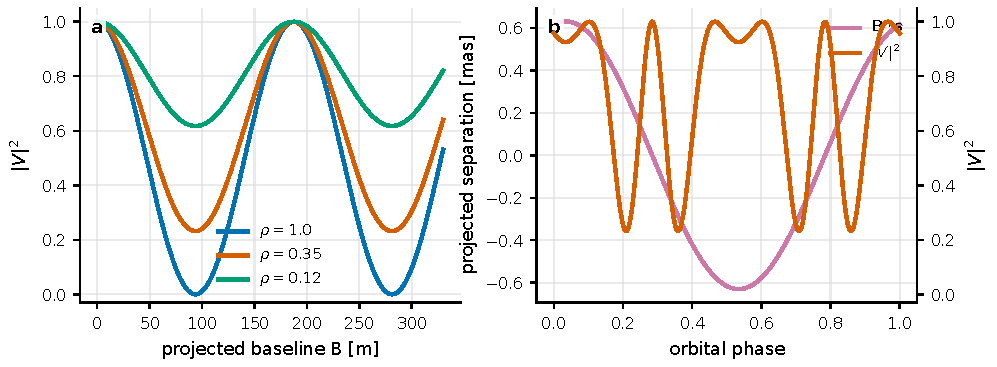
\includegraphics[width=0.96\linewidth]{figures/generated/chapter_20/ch20_binary_visibility.pdf}
\caption{The binary \(|V|^2\) case. The left panel shows how, at fixed angular separation, the flux ratio \(\rho\) controls the depth of the oscillation with baseline; the right panel shows how, in an inclined orbit, the projected separation \(\bm B\!\cdot\!\bm s\) varies with orbital phase, thereby changing \(|V|^2\) on a fixed baseline. Multi-baseline and multi-epoch data are used to separate the separation, the flux ratio, and the orbital geometry.}
\label{fig:e26-binary}
\end{figure}

\section{The correlator: turning the event table into a correlation function, and learning to doubt it}
\label{sec:e26-correlator}

The previous sections silently assumed ``we already have \(g^{(2)}(\tau)\).'' This section fills in the intermediate machine, the \textbf{correlator}, and stresses that half its value lies in \textbf{quality control}, not speed.

The correlator's task is a single sentence: turn two event tables into a batch of delay histograms, with every coincidence pair traceable back to the two original events and one time difference. There are three routes to implement it, all computing the same quantity but at different costs. The crudest double loop compares all event pairs, with computation growing as \(N_1 N_2\), absurdly slow. If events are already time-sorted, one compares only neighbors falling within the correlation window \(|t_j-t_i|<\tau_{\max}\), and the computation drops to about \(N_\gamma k\), where \(k\sim2R\tau_{\max}\) is the number of candidate pairs near each photon. The third route first projects events onto uniform time bins into a sequence, then does the cross-correlation via fast Fourier transform, with computation about \(M\log M\) (\(M=T/\Delta t\)). The three give consistent results, but their memory footprint, time resolution, and dead-time handling differ; this itself is a good comparison experiment.

Why is the engineering pressure so great? Two scalings explain everything. The \textbf{number of baselines} of a multi-telescope array grows quadratically with the number of telescopes (Chapter \ref{chap:e11}): 4 telescopes have only 6 baselines, but 60 have \(\binom{60}{2}=1770\). A single telescope's \textbf{raw data rate} swells as the time bin narrows and the spectral channels multiply:
\begin{equation}
  D\simeq \frac{N_\nu\,n_{\rm bit}}{\Delta t},
  \label{eq:e26-datarate}
\end{equation}
\begin{formulaexplain}
\(D\) is the single-stream data rate, \(N_\nu\) is the number of spectral channels retained simultaneously, \(n_{\rm bit}\) is the number of bits per time bin, and \(\Delta t\) is the time-bin width. The narrower the bin and the more the channels, the fiercer the data stream: this determines what hardware the correlation must lean on.
\end{formulaexplain}
Grounding the units: \(D\) has units \(\mathrm{bit\,s^{-1}}\), \(N_\nu\) is dimensionless, \(n_{\rm bit}\) is dimensionless, and \(\Delta t\) has units s. Plug in real numbers: with \(\Delta t=4\,\mathrm{ns}\), single channel \(N_\nu=1\), \(n_{\rm bit}=16\), \(D\simeq16/(4\times10^{-9})=4\times10^{9}\,\mathrm{bit\,s^{-1}}=4\,\mathrm{Gb\,s^{-1}}\); retaining 64 spectral channels at once, a single telescope surges to \(256\,\mathrm{Gb\,s^{-1}}\). This is why modern intensity interferometry is inseparable from GPU/FPGA real-time correlation, tiered triggering, on-chip accumulation, or strict compression: MAGIC's real-time dead-time-free correlator and VERITAS's online/offline pipelines were both forced into being by this data rate \citep{2020NatAs...4.1164A,2024MNRAS.529.4387A,2024ApJ...966...28A}.

\begin{figure}[tbp]
\centering
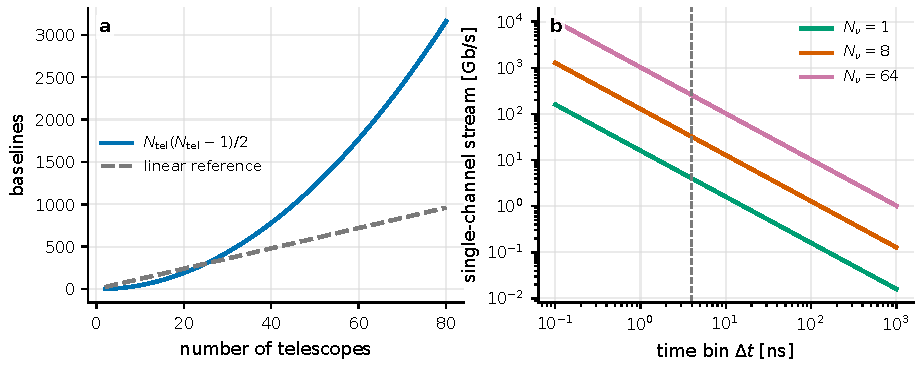
\includegraphics[width=0.96\linewidth]{figures/generated/chapter_20/ch20_correlator_scaling.pdf}
\caption{The two scalings of a multi-telescope correlator. Left: the number of baselines grows quadratically with the number of telescopes, so expanding the array rapidly increases the correlation load. Right: the single-stream data flow rises as the time bin narrows and the spectral channels multiply; nanosecond sampling plus tens of spectral channels has already entered the regime that must be handled by real-time hardware or GPUs.}
\label{fig:e26-correlator}
\end{figure}

What truly sets this section apart from the earlier ones is the \textbf{null test}, and it should be graded as seriously as the result plots, not a token in the appendix. At minimum one should do these: shift the second stream as a whole by a time far greater than \(\tau_c\), and the real peak \textbf{must vanish}; cap the light or run the same pipeline with no starlight, and electronics crosstalk \textbf{should not} produce a zero-delay peak; scramble the polarization or spectral channels, and only the physically correlated channel should retain signal; slice the data by time, and \(\hat g^{(2)}(0)-1\) should converge smoothly as \(T^{-1/2}\) with integration time, rather than concentrating in one short segment. These tests directly determine whether a peak can be interpreted as an astronomical signal: the tabletop/in-sky experiments of Guerin et al., the photon-counting schemes of AQuEye/IquEye, and the intensity interferometry of modern Cherenkov arrays all treat them as part of the result \citep{2017MNRAS.472.4126G,2016SPIE.9907E..0NZ,2021MNRAS.506.1585Z,2020NatAs...4.1164A}. \textbf{One line of discipline}: a small peak that passes the null test is worth far more than a big peak that does not.

\section{Numerically demonstrating SPADE: the information is not in the brightest pixel}
\label{sec:e26-spade}

Now switch to a seemingly unrelated but actually cognate experiment, echoing Chapter \ref{chap:e12}. Earlier we used long baselines to reach high spatial frequencies; here the question is reversed: \textbf{we have already imaged, and two point sources sit closer than the point-spread function; can we still measure their separation?} The answer from direct imaging is disheartening, but mode sorting (SPADE) will tell you the information was there all along: just not in those few bright pixels you were staring at.

First the picture. Two equal-brightness, incoherent point sources with separation \(s\) far smaller than the point-spread-function (PSF) width \(\sigma\) produce a combined image in the focal plane that is almost just ``a little bit fatter.'' The trouble is that the \textbf{derivative} of the pixel intensity with respect to \(s\) tends to zero as \(s\to0\): the parameter you want to estimate barely changes what you measure, so the Fisher information collapses toward zero. This is the statistically precise meaning of the \textbf{Rayleigh curse}: not ``cannot be resolved,'' but ``the measurement mode of direct imaging wastes the information about \(s\)'' \citep{2015Optic...2..646T,2016PhRvX...6c1033T}.

SPADE uses a different measurement: not measuring pixel intensity but projecting the light onto a set of \textbf{Hermite--Gaussian modes} and counting the photons in each mode. For a Gaussian PSF and equal-brightness two-point sources, this is the known result of Chapter \ref{chap:e12}: the probability of landing in the \(n\)-th mode is Poisson-shaped:
\begin{equation}
  p_n=e^{-\Gamma}\,\frac{\Gamma^{\,n}}{n!},\qquad
  \Gamma=\left(\frac{s}{4\sigma}\right)^{\!2}.
  \label{eq:e26-spade-prob}
\end{equation}
\begin{formulaexplain}
\(p_n\) is the probability that a photon is projected onto the \(n\)-th Hermite--Gaussian mode, with \(n=0,1,2,\dots\) the transverse mode index. \(\Gamma\) is a dimensionless small quantity blending the separation with the PSF width. The smaller the separation, the smaller \(\Gamma\), and the vast majority of photons still land in the fundamental mode \(n=0\); but the little bit of probability of \(n\ge1\) is extremely sensitive to \(s\).
\end{formulaexplain}
Grounding the symbols: \(s\) is the angular separation (in the same angular units as \(\sigma\), or the same focal-plane length units), \(\sigma\) is the Gaussian PSF width, and \(\Gamma\), \(p_n\) are dimensionless. Plug in numbers: at \(s=0.2\sigma\), \(\Gamma=(0.2/4)^2=2.5\times10^{-3}\), so \(p_1\approx\Gamma=2.5\times10^{-3}\), and only two or three out of a thousand photons make it into the \(n=1\) mode, but it is precisely these two or three photons that carry almost all the information about \(s\).

Why does the information not collapse? Compute the Fisher information of the Poisson probability \eqref{eq:e26-spade-prob} step by step. The Fisher information of a single photon about the parameter \(s\) is
\[
  I_{\rm SPADE}(s)=\sum_{n}\frac{1}{p_n}\!\left(\frac{\partial p_n}{\partial s}\right)^{\!2}.
\]
Using a standard fact about the Poisson distribution, the Fisher information of the Poisson mean \(\Gamma\) itself is \(1/\Gamma\), together with the chain rule \(I_s=(d\Gamma/ds)^2\cdot(1/\Gamma)\). Substituting \(\Gamma=s^2/(16\sigma^2)\), so \(d\Gamma/ds=s/(8\sigma^2)\), we get
\[
  I_{\rm SPADE}(s)=\frac{\big(s/8\sigma^2\big)^2}{s^2/(16\sigma^2)}
  =\frac{s^2/(64\sigma^4)}{s^2/(16\sigma^2)}=\frac{16\sigma^2}{64\sigma^4}=\frac{1}{4\sigma^2}.
\]
Not a step skipped, and the result is astonishingly clean: \(I_{\rm SPADE}=1/(4\sigma^2)\), \textbf{independent of the separation \(s\)}: even as \(s\to0\), the information carried by each photon does not decay. By contrast, the Fisher information of direct imaging collapses toward zero as \(s\to0\). This is the whole secret of how SPADE crosses the Rayleigh curse.

\begin{figure}[tbp]
\centering
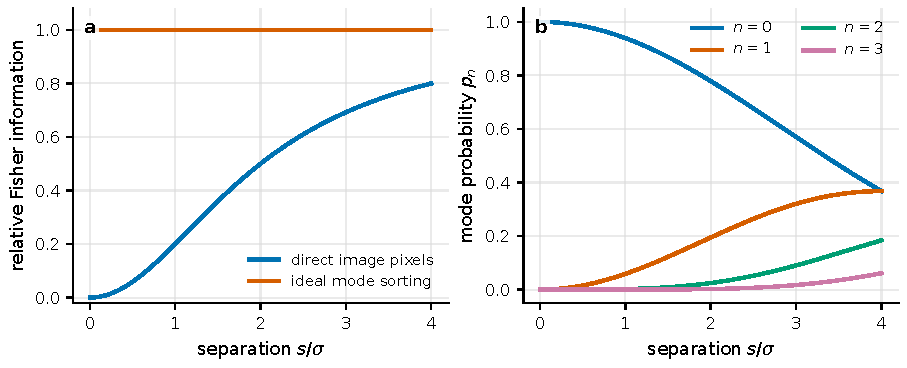
\includegraphics[width=0.96\linewidth]{figures/generated/chapter_20/ch20_spade_computational_experiment.pdf}
\caption{The SPADE computational experiment. The left panel compares the relative Fisher information of direct pixel imaging and ideal mode sorting at small separation: direct imaging loses information as \(s/\sigma\ll1\), while mode sorting stays near constant. The right panel shows the Hermite--Gaussian mode probabilities; at very small separation the higher-mode probabilities are small but have nonzero slope, so a highly stable, low-crosstalk mode measurement is required.}
\label{fig:e26-spade}
\end{figure}

\textbf{A pitfall you must write into the code}: the pretty constant curve above is the \textbf{ideal} case. In a real system, the mode basis does not perfectly match the true PSF, the centering has errors, there are aberrations, and there is background light: any \textbf{mode crosstalk} lets a bit of the light that should be in the clean \(n=1\) mode leak into \(n=0\), thereby laying down an \textbf{information floor} for the Fisher information and flattening the \(s\to0\) advantage. So teaching code should not plot only the ideal curve but add a tunable crosstalk parameter, letting students watch the information floor rise as the crosstalk increases. For precisely this reason, SPADE is currently better suited as a computational experiment and pathfinder than as a promise that the next-generation telescope can losslessly reach the quantum limit \citep{2016OExpr..24.3684N,2017PhRvL.118g0801T}.

\section{Capstone project: how the Type Ia distance toy model strings together the whole error budget}
\label{sec:e26-typeia}

The final project assembles the previous parts into a whole machine, and deliberately exposes the danger a toy model most easily conceals: angular radius, velocity, and explosion time look as if they differ only by a proportionality constant, but the real errors come from \textbf{different instruments, different models, different epochs}. This is the idea of using the expanding-photosphere method to measure the angular-diameter distance of a Type Ia supernova \citep{2025PhRvD.111h3047K}.

The physical chain is this: the spectral model gives the photospheric expansion velocity \(v_{\rm ph}(t)\), intensity interferometry gives the photospheric angular radius \(\theta_{\rm ph}(t)\), and comparing the two yields the angular-diameter distance:
\begin{equation}
  \theta_{\rm ph}(t)=\frac{R_{\rm ph}(t)}{D_A}\simeq\frac{v_{\rm ph}\,(t-t_0)}{D_A}.
  \label{eq:e26-typeia-theta}
\end{equation}
\begin{formulaexplain}
\(\theta_{\rm ph}\) is the photospheric angular radius, \(R_{\rm ph}\) is the physical radius, \(D_A\) is the angular-diameter distance, and \(t_0\) is the explosion time. If the photosphere expands at approximately constant velocity \(v_{\rm ph}\), the physical radius is about velocity times time; dividing it by the angular radius extracts the distance.
\end{formulaexplain}
Grounding the symbols and dimensions: \(v_{\rm ph}\) has units \(\mathrm{cm\,s^{-1}}\), about \(8\times10^8\)--\(1.5\times10^9\,\mathrm{cm\,s^{-1}}\) for a normal Type Ia at early times; \(t-t_0\) has units s or d, and intensity interferometry is most interested in a few days to a few tens of days after explosion; \(D_A\) is in Mpc; and \(\theta_{\rm ph}\) is usually a few to a few tens of \(\mu\mathrm{as}\). Plug in real numbers: \(v_{\rm ph}=10^{9}\,\mathrm{cm\,s^{-1}}\), \(t-t_0=15\,\mathrm{d}=1.30\times10^{6}\,\mathrm{s}\), the physical radius \(R_{\rm ph}\approx1.30\times10^{15}\,\mathrm{cm}\); then take \(D_A=20\,\mathrm{Mpc}=6.17\times10^{25}\,\mathrm{cm}\),
\[
  \theta_{\rm ph}\approx\frac{1.30\times10^{15}}{6.17\times10^{25}}\ \mathrm{rad}
  \approx2.1\times10^{-11}\,\mathrm{rad}\approx4.3\,\mu\mathrm{as}.
\]
At \(\lambda=500\,\mathrm{nm}\), this corresponds to a first-zero baseline scale \(\lambda/\theta\sim24\,\mathrm{km}\). If one is willing to use the whole visibility curve rather than only wait for the first zero, kilometer-to-ten-kilometer baselines still have science to mine, but the error budget is stretched extremely tight.

How do we combine the angular radius and velocity into a distance posterior? Write a joint likelihood that simultaneously penalizes the inconsistency of the ``angular-radius prediction'' and the ``velocity prediction'':
\begin{equation}
  \ln{\cal L}(D_A)=
  -\frac12\sum_k\!\left[\frac{\hat\theta_k-v_{{\rm ph},k}(t_k-t_0)/D_A}{\sigma_{\theta,k}}\right]^2
  -\frac12\sum_k\!\left[\frac{\hat v_k-v_{{\rm ph},k}}{\sigma_{v,k}}\right]^2 .
  \label{eq:e26-typeia-like}
\end{equation}
\begin{formulaexplain}
\(D_A\) is the distance to be estimated, \(\hat\theta_k\) and \(\hat v_k\) are the angular radius and velocity measured at the \(k\)-th epoch, and \(\sigma_{\theta,k}\), \(\sigma_{v,k}\) are their respective errors. The first sum enforces ``the angular radius must match \(v(t-t_0)/D_A\),'' and the second enforces ``the velocity model must match the measured velocity.'' Minimizing both together is what constrains \(D_A\).
\end{formulaexplain}
Grounding the symbols: \(\hat\theta_k\) comes from the \(|V|^2\) fit of the \(k\)-th epoch (the machinery of Eqs.\ \eqref{eq:e26-v2-estimator}, \eqref{eq:e26-uniform-disk}), with units rad or \(\mu\mathrm{as}\); \(\hat v_k\) comes from spectral-line velocity or a radiative-transfer model, with units \(\mathrm{cm\,s^{-1}}\); and \(\sigma_{\theta,k}\), \(\sigma_{v,k}\) each \textbf{simultaneously} contain statistical error and model systematic error. \textbf{The biggest pitfall of the toy model} is right here: if you lazily add only a \(10\%\) Gaussian noise to \(\hat\theta\), you will get a posterior so narrow it is distorted. A real project must have students turn those ``invisible knobs'': vary the explosion time \(t_0\), add a velocity gradient, put in non-spherical asymmetry, replace the uniform disk with a limb-darkened brightness distribution, and then watch the posterior widen bit by bit. The posterior \textbf{should} widen; that is what an honest error budget looks like.

\begin{figure}[tbp]
\centering
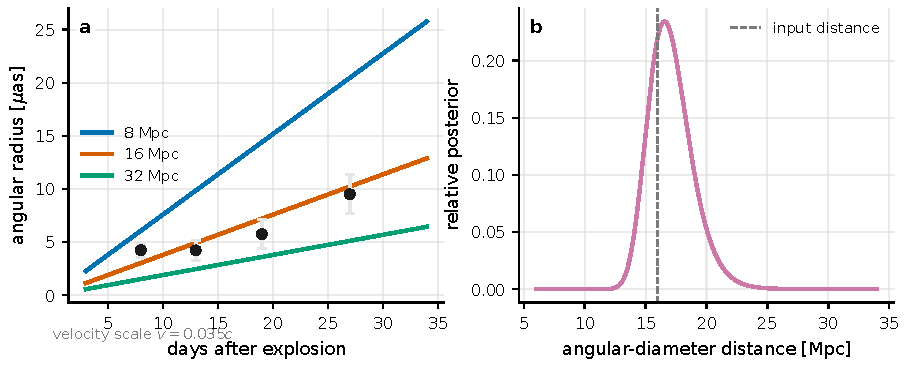
\includegraphics[width=0.96\linewidth]{figures/generated/chapter_20/ch20_typeia_distance_posterior.pdf}
\caption{The Type Ia supernova angular-diameter-distance toy model. The left panel uses a simplified expansion model with \(v_{\rm ph}=0.035c\), giving the angular radius versus time at various distances, with simulated angular-radius measurements overlaid; the right panel combines these angular radii with the velocity model into a \(D_A\) posterior. A real analysis must replace the constant-velocity shell with a radiative-transfer model, and write non-spherical asymmetry, the line-forming layer, and the baseline coverage into the error budget.}
\label{fig:e26-typeia}
\end{figure}

These five projects strung together are exactly a course line of increasing difficulty: first use an LED, pseudothermal light, and a laser to measure \(g^{(2)}(\tau)\), verifying Poisson and bunching; then practice time-shift background, quality selection, and \(T^{-1/2}\) convergence on the same event table; enter spatial coherence and fit the \(|V|^2\) of a uniform disk and a binary, feeling the role of baseline coverage; then do SPADE, seeing how the Fisher information escapes the Rayleigh curse and how it is pressed back to the floor by crosstalk; and finally use the Type Ia toy model to propagate together the uncertainties of angular radius, velocity, and explosion time. Each project's deliverables are equally plain: one event-table description, one runnable script, a set of plots, one short report citing real literature, and \textbf{at least two null tests}. Remember the line that recurs throughout this chapter: code that runs is only the first hurdle; a plot that cannot account for its time reference, \(\beta\) calibration, crosstalk matrix, or systematic error can be generated, but cannot be treated as an astronomical measurement.

\section*{Chapter Summary}
\addcontentsline{toc}{section}{Chapter Summary}

\begin{itemize}
  \item \textbf{Everything begins with the event table.} Each photon leaves a time, a channel, a polarization, and a quality flag; the light curve is only one lossy projection of it (Eq.\ \eqref{eq:e26-binned-count}). Bin first, and you can never go back.
  \item \textbf{Poisson's signature is variance equals mean.} Use the Fano factor \(F=\operatorname{Var}/\langle N\rangle\to1\) to test shot noise (Eq.\ \eqref{eq:e26-fano}); \(F<1\) is often dead-time disguised as antibunching, not new physics.
  \item \textbf{Bunching is seen via coincidence excess, but gets diluted.} \(\hat g^{(2)}\) is normalized by the time-shift background (Eq.\ \eqref{eq:e26-g2-estimator}); when the coherence time is far smaller than the response width, the thermal-light peak shrinks by \(\tau_c/\Delta\tau\) to the \(10^{-5}\) level.
  \item \textbf{Visibility is the object's Fourier fingerprint.} \(|V|^2\) is obtained from \(\hat g^{(2)}(0)-1\) divided by the instrument contrast \(\beta\) (Eq.\ \eqref{eq:e26-v2-estimator}); \(\beta\) is in the denominator, so its calibration error is directly amplified. The uniform-disk first zero \(B_{\rm null}\approx1.22\lambda/\theta\) (Eq.\ \eqref{eq:e26-uniform-disk}), and a \(1\,\mathrm{mas}\) bright star is at about a hundred-meter baseline.
  \item \textbf{Multiple baselines, multiple epochs are for breaking degeneracies.} The binary's oscillation half-amplitude \(2\rho/(1+\rho)^2\) (Eq.\ \eqref{eq:e26-binary}) shallows as the companion dims; single-direction uv coverage gives an elongated, misleading error ellipse.
  \item \textbf{Half the correlator's value is the null test.} Time shift, capping, channel scrambling, and \(T^{-1/2}\) convergence must all be graded like the results; the data-rate scaling (Eq.\ \eqref{eq:e26-datarate}) explains why real-time hardware is a must.
  \item \textbf{SPADE frees information from the bright pixels.} The mode probabilities are Poisson-shaped (Eq.\ \eqref{eq:e26-spade-prob}), and the Fisher information \(1/(4\sigma^2)\) is independent of separation; but crosstalk lays down an information floor, so the ideal curve cannot be trusted lightly.
  \item \textbf{The capstone tests the error budget, not the fit.} In the Type Ia distance toy model (Eqs.\ \eqref{eq:e26-typeia-theta}, \eqref{eq:e26-typeia-like}), the posterior \textbf{should} widen once you put in real systematic errors; if it does not, you have not yet put the danger in.
\end{itemize}

\medskip
\noindent\textbf{Questions to Ponder:} (1) You measure \(F=0.7\); give at least two physically distinct explanations, and design an experiment to distinguish each pair. (2) If a binary's companion flux ratio drops from \(\rho=0.3\) to \(\rho=0.05\), by roughly what factor must the accidental-coincidence count \(H\) increase to maintain the same oscillation significance? (3) Adding \(1\%\) mode crosstalk in SPADE, to what order of magnitude does the information floor push up the smallest resolvable \(s/\sigma\)?
